% v2-acmtog-sample.tex, dated March 7 2012
% This is a sample file for ACM Transactions on Graphics
%
% Compilation using 'acmtog.cls' - version 1.2 (March 2012), Aptara Inc.
% (c) 2010 Association for Computing Machinery (ACM)
%
% Questions/Suggestions/Feedback should be addressed to => "acmtexsupport@aptaracorp.com".
% Users can also go through the FAQs available on the journal's submission webpage.
%
% Steps to compile: latex, bibtex, latex latex
%
% For tracking purposes => this is v1.2 - March 2012
\documentclass{acmtog} % V1.2
\usepackage{algpseudocode,algorithm,algorithmicx, graphics}


%\acmVolume{VV}
%\acmNumber{N}
%\acmYear{YYYY}
%\acmMonth{Month}
%\acmArticleNum{XXX}
%\acmdoi{10.1145/XXXXXXX.YYYYYYY}

\acmVolume{Unpublished}
\acmNumber{}
\acmYear{2016}
\acmMonth{December}
\acmArticleNum{}
\acmdoi{}

\begin{document}

	\title{Parallel Data Mining} % title
	
	\author{JASON MA {\upshape and} KANISHK TANTIA
		\affil{Harvey Mudd College}}
		% NOTE! Affiliations placed here should be for the institution where the
		%       BULK of the research was done. If the author has gone to a new
		%       institution, before publication, the (above) affiliation should NOT be changed.
		%       The authors 'current' address may be given in the "Author's addresses:" block (below).
		%       So for example, Mr. Fogarty, the bulk of the research was done at UIUC, and he is
		%       currently affiliated with NASA.
	

	
	\maketitle
	\section{Abstract}
	There is currently vast interest in both, High Performance Parallel Computing and in Deduplication efforts to save space and reduce memory usage. While deduplication methodology is still in it's infancy, a major target for improvement are the "Chunking" algorithms that take in file or block level traces and identify candidate blocks that may be similar to each other across the trace. These chunking algorithms are primarily serial in nature, due to the serial, interconnected nature of block and file traces. In this paper we propose a parallelized version of a commonly used Chunking algorithm based on the Rabin method, dubbed "Rabin Context Defined Chunking" or RabinCDC. The key idea behind Parallel RabinCDC is to apply data parallelism to the trace to apply the cyclic nature of RabinCDC to different sections of the trace without introducing large differences in breakpoints across trace data. We use multiple processes to carry out a serialized version of RabinCDC on multiple sections of the trace which are broken apart in a context defined manner. We further compare parallel RabinCDC to FastCDC, an industry standard serial chunking algorithm, to Serial RabinCDC, and to AECDC, a now defunct chunking algorithm. Our comparisons show large speed and efficiency improvements over the serial CDC algorithms over large traces with multiple processes running. Parallel RabinCDC also had few differences in the identified break points, which ensures that the deduplication ration remains nearly identical.
	
	\section{Introduction}
	Data storage needs have grown exponentially as more data is increasingly digitized. IBM estimates that 2.5 Quintillion bytes of data are created daily. IDC research estimates that digital data growth will grow at a compound growth rate of 11.7\% through 2020. As of 2011, the demand for more storage has outpaced the growth of digital storage means, and by 2020, it is estimated that the demand will outpace the growth of digital storage by over 15,000 Exabytes of data per year. \\
		
		Data Deduplication is an efficient manner in which data usage can be reduced, and has slowly gained traction over the last decade. Assuming that a large amount of the data being stored is redundant or "junk" data, data storage needs can be met by simply never storing multiple copies of data and instead just providing the same set of bytes when the data is required. Data deduplication therefore removes redundant data at a file or chunk level, and uses a hash code to identify similar blocks, which are then compared in order to eliminate redundancies while salvaging important data. \\
		
		A critical requirement of data deduplication is efficient chunking, which involves looking at traces of data and identifying blocks of data that may be similar to each other. The research standard for chunking is at the block level, as this allows for the data stream to be fine tuned and allows for deduplication to proceed at a much finer granularity. Chunk level deduplication has been explored by various authors. The simplest method, which is not considered in this paper due to it's lack of practical application, is Fixed Size Chunking [Quinlan et. al]. Since FSC is unable to actually account for slight shifts in data, and changes every subsequent breakpoint after a small change in files due to a cascading effect, it has been considered defunct for a while. This is an example of a \textit{boundary shift} problem [Muthitacharoen], which is an unwanted shift in data that has not been modified through either an insertion or deletion.\\
		Context Defined Chunking, (CDC), is a solution to the \textit{boundary shift} problem. CDC methods declare chunk boundaries on the basis of only the data contained within each block, and therefore performs some preliminary block analysis before declaring a breakpoint. This has the drawback of a higher CPU overhead, but the advantage of avoiding cascading shifts due to small modifications. Moreover, the preliminary analysis also allows for a higher deduplication ration, as the fast analysis allowed for by CDC methods ensure that blocks need to meet certain criteria based on their content. \\
		
		The more complex CDC methods considered are RabinCDC [Rabin], FastCDC, [Wen et al] and AECDC [Zhang, Yucheng at. al]. These methods are currently industry standard, except for AECDC, and are all highly effective at detecting context defined breakpoints. Each of these methods is considered to be accurate at identifying candidate blocks for deduplication, but, with the exception of FastCDC, each has a high CPU Overhead. FastCDC is a sequential algorithm that was specifically designed to have a low CPU Overhead, but has a worse deduplication ration than RabinCDC and AECDC.\\
		
		CDC methods are sequential in nature, since they run through the trace and identify breakpoints based on each line of the trace. FastCDC specifically is extremely trace dependent, and is impossible to parallelize without causing a significant cascade effect in the breakpoints. However, RabinCDC is cyclic in nature, and judges each block of data by hashing it and comparing it to stored hash values, using a cyclic and rolling hash algorithm. \\
		
		In general, we observe that none of the current CDC methods are parallelized. While algorithms like FSC do not require parallelization, as they are simplistic enough to perform well without any added parallelization, it is certainly necessary for CDC methods, which judge traces based on block data, and therefore have an overall O(n) time at best. Given that trace data routinely reaches very large sizes, parallelization could certainly improve the Big O time of these algorithms, while changing the output very little.Motivated by this observation, we proposed Parallel RabinCDC, which has the following characteristics:
		
		\begin{itemize}
		\item \textbf{Task Parallelism}: Parallel RabinCDC is a wrapper that runs the sequential RabinCDC algorithm on multiple processes, thus reducing Big O time to O($\frac{n}{p}$)
		\item \textbf{Efficient Hashing}: Parallel RabinCDC uses a simple cyclic hash, similar to the FastCDC hash methodology, in order to increase hashing time on each parallel processor 
		\end{itemize}
		
		We see that there is a linear improvement in processing speed under Parallel RabinCDC vs number of Processors, and that the strong and weak scaling are both linear in nature. We further observe that the Parallel RabinCDC algorithm is modular in nature, and would be trivial to implement in research involving the current sequential version assuming that Parallel Processing capabilities are enabled.\\
		
		The rest of this paper is laid out as follows. Section 3 presents background information that is necessary for this research. Section 4 discusses the design of Parallel RabinCDC algorithm. Section 5 discusses testing Methodology and trace data. Section 6 presents an evaluation of the experimental work. Section 7 presents results on practical and synthetic trace data. Section 8 discusses future work and conclusions.
		
	\section{Background}
	\subsection{General Chunking}
	Chunking, as mentioned, is the first step in data deduplication, and primarily breaks large traces into smaller blocks that can then be compared in order to identify duplicates. Fixed Size Chunking [Quinlan] has a low CPU overhead and is extremely fast, but also inaccurate. It is unable to handle \textit{boundary shift} problems, so that any insertions or deletions in a file cause a cascading effect that disrupt every breakpoint after the modification. 

	\subsection{FastCDC}

	FastCDC was first proposed in 2016 [Wen et al]. It involves a simplistic hash judgement mechanism and an efficient bit-shifting hashing algorithm that increases hashing speed. FastCDC is currently considered to be an industry standard chunking algorithm. \\
	
	FastCDC first generates a random 1:1 mapping of every 8 bit number to a random value in a hash table. It then runs through the trace, and accounts for each block number in a running total, with upper and lower bounds on block size. The block number first undergoes a bit shift, and then the bit-shifted value is looked up in the hash table. The looked up value is added to a running total, and once the running total is divisible by a given value, a breakpoint is designated [Wen et al.]\\
	
	Unfortunately, FastCDC is very difficult to parallelize as the granularity of the tasks that we can run in parallel are too small to see much benefit overall compared to running it serially. However, it is a good upper bound or "golden standard" for algorithmic runtime. 
	
	\subsection{RabinCDC}
	RabinCDC involves a cyclic, rolling hash. Proposed by Rabin as a simple algorithm in 1981 for the identification of similar substrings, it has been modified to work for block addresses. Rabin is a variable or Dynamic chunking algorithm, which has a \textit{window} of certain size. Every time the contents of the window match a predefine criteria, a breakpoint is introduced. If this fails to happen, the window moves forward by one byte and the process repeats.\\
	
	The Rabin Rolling Hash we designed works in the following way. The window of size \textit{n} is summed, and bit shifted by 1 to the left. The bit-shifted sum is then modded against a prime number generated by random seed, and if the resulting value is 0, a breakpoint is introduced. This is a modified version of the original Rabin Fingerprint, which was found to produce similar results to the original Rabin Algorithm, as per the PCompress Project.\\ 

	Unlike FastCDC, RabinCDC is a slower algorithm. However, it is extremely parallelizable, because it guards against insertions and deletions due to the cyclic property of the hashing algorithm. As the hashing algorithm doesn't depend on past block addresses, but simply on the current \textit{n} valid bytes, splitting up the trace means that the breakpoints are largely unaffected. Considering the likelihood of a cascading effect is extremely low, RabinCDC is perfect for parallelization.\\
	
	The sequential version of RabinCDC is used to provide a primary lower bound for the parallel version, and provides information on the improvement from control that is visible post-parallelization.\\
	
	\subsection{AECDC}
	Asymmetric Extremum Chunking, or AE CDC was introduced in 2015 [Zhang et al.] AE CDC is fast, but is still slower than RabinCDC and FastCDC, while being upto 3x more accurate.\\
	
	AE CDC depends on extreme values and two candidate windows. The first window of size \textit{n} contains bytes behind a candidate block address. The second window of size \textit{m} contains the bytes immediately ahead of a candidate block address. Each new block address is considered a viable breakpoint, and is eliminated as a breakpoint if it does not meet both the following criteria:
	
	\begin{itemize}
	\item The block address must have a value greater than any block address seen in the \textit{tail} window.
	\item The block address must be greater than or equal to any block address in the \textit{head} window.
	\end{itemize}
	
	AE CDC is a slightly slower algorithm than RabinCDC or FastCDC. Thus, it is apparent that this algorithm will provide a useful lower bound of how slow our parallelization will affect Rabin CDC.

	\section{Data}
	\subsection{Practical Trace Data}
	We used practical trace data from the work of Kanishk and Kuenning from the summer of 2016. \\
	\subsection{Synthetic Trace Data}
	In order to gain a more complete understanding of parallelization improvements, we synthesized trace data using a simple Markov Chain on the practical data. We generate this new file using an aggregated file of our practical trace data as a source. The size of the chunks with which we sampled the source files ranged from 1 line to 20 lines. This method allows us to maintain patterns from the data it is sampled from while allowing tests at large volumes. Thus, we can more carefully tune our tests to our specific requirements, and test conditions outside of what the practical trace data covers. Additionally, the randomness of the index from which we sample and the size of the chunk we sample out allows us to maintain randomness in our testing data to mimic real world situations.\\
	
	For our testing, we created files that are 1 million to 10 million lines. We increment the file sizes by 1 million lines. These file sizes will be adequate in covering the full behavior our parallelized RabinCDC at small file sizes, and its behavior as the file sizes approach infinity, which let's us analyze the O(n) behavior. Additionally, the choices for which sizes we used were chosen, so that the weak scaling efficiency could also be easily tested.
	
	We considered the possibility of testing even larger file sizes, but the process of generating these files were deemed to take too long, and our results may be over fitted to the practical trace data we have. If given more practical trace data and a better system to test on, we will consider more intensive stress testing.
	
	
	\section{Experiments}
	We tested our algorithms in a Python3 environment, using the \texttt{multiprocessing} module to implement parallelization. We will note that this only creates multiple processes, and allows the CPU's scheduler to handle the parallelization of these processes, but these results are still valid in that they show how one can easily parallelize any algorithm for significant runtime improvement. The required Python modules we used for testing were \texttt{multiprocessing} for parallelizing, \texttt{time} for timing our algorithm performance, \texttt{random} for data generation, and \texttt{matplotlib.pyplot} for graphing purposes. 
	
	Our testing system is a Windows Surface Pro 3 with an Intel(R) Core(TM) i5-4300 CPU @ 1.90 GHZ. It has 2 Cores and 4 logical processors with cache sizes of 128 KB, 512 KB, 3.0 MB for the L1, L2, and L3 cache respectively. We considered the possibility of using Comet for testing, but due to incompatibility issues, we decided against using Comet. This system is adequate for showing that any individual can parallelize their algorithms. 

	
	
		\begin{figure}
			\centerline{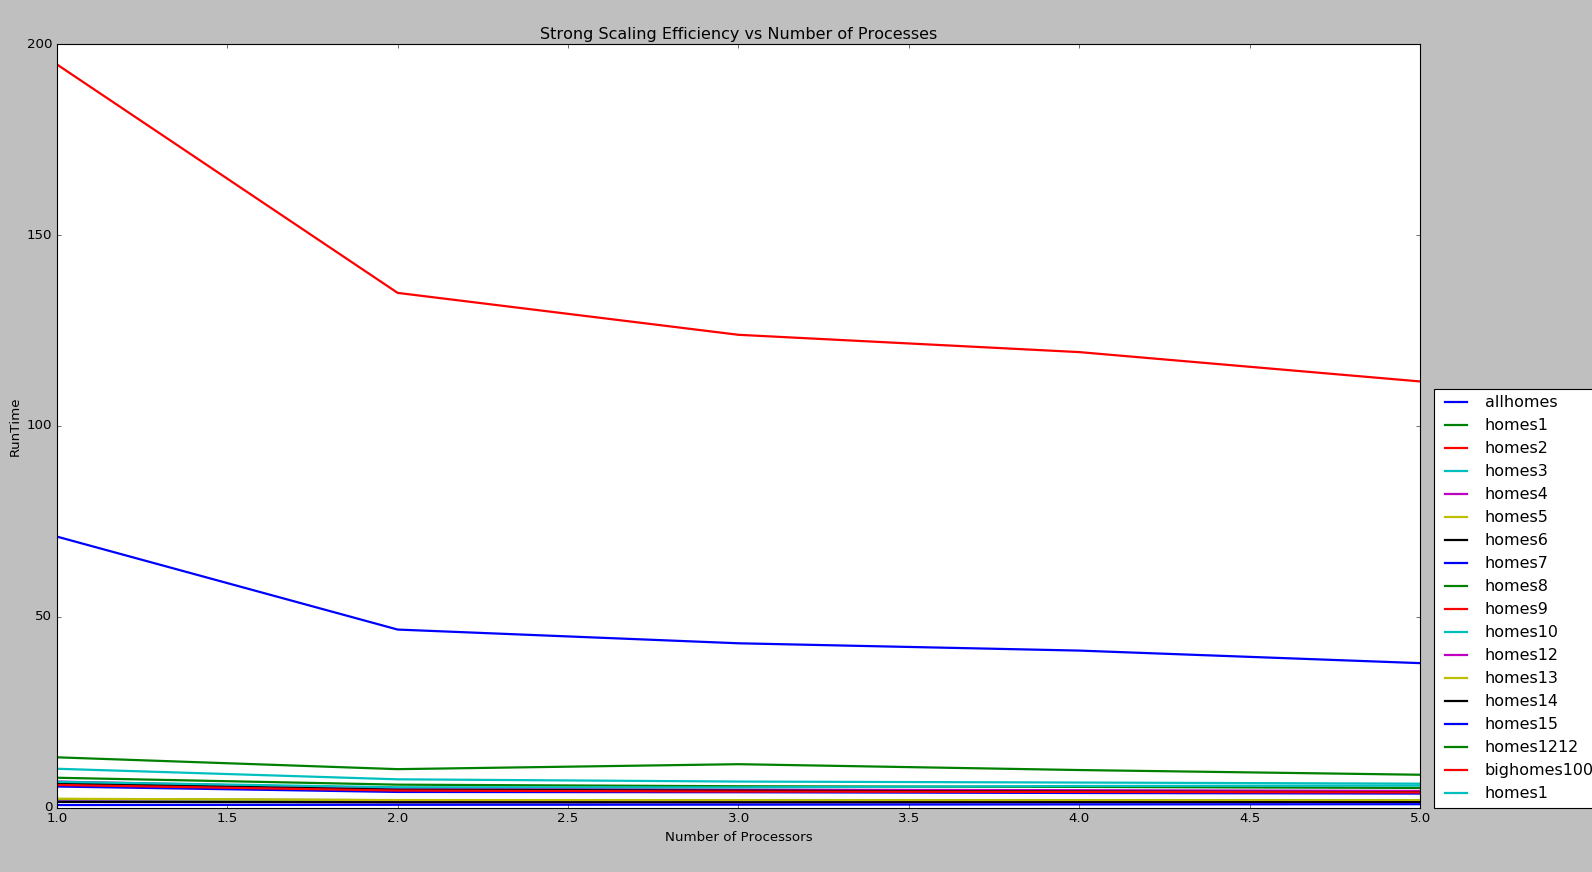
\includegraphics[width=8.5cm]{img/AllTimesvsProcess}}
			\caption{Graph showing total runtime vs number of processes}
			\label{fig:runtimecomparisons}
		\end{figure}
	\subsection{Practical Trace Data Tests}

	With the practical trace data, we timed the run time over 10 tests using from 1 process to 5 processes. Given the uneven size of these files, it is only feasible to test the strong scaling efficiency.
	\subsection{Synthetic Trace Data Tests}
	With data that we can generate, we gain much better control over the types of tests that we can run. Thus, using synthetic trace data, we can specifically target the strong and weak scaling efficiency of a parallel Rabin CDC algorithm. To generate data, we run the tests 10 times and average the time across all the runs to produce an average run time. \\
	
	To test the strong scaling of our parallelization, we ran our algorithm on the test data serially, and then increased the number of processors up to 5. We time how long it takes in each case, starting from when the algorithm is passed the data in the serial case and starting from when we create the new processes in the parallel case. Our tests ranged from files that were 1 to 10 million lines long. Using these results, we can uncover how well parallelization affects Rabin CDC at small to large file sizes.\\
	
	To test the weak scaling efficiency, we also created file sizes ranging from 1 to 5 million lines long. We then ran our CDC algorithms on these files keeping a constant ratio of 1 million lines to one process. \\ 
	
	\section{Results}
	\subsection{Strong Scaling Efficiencies}

	
	\begin{figure}
				\centerline{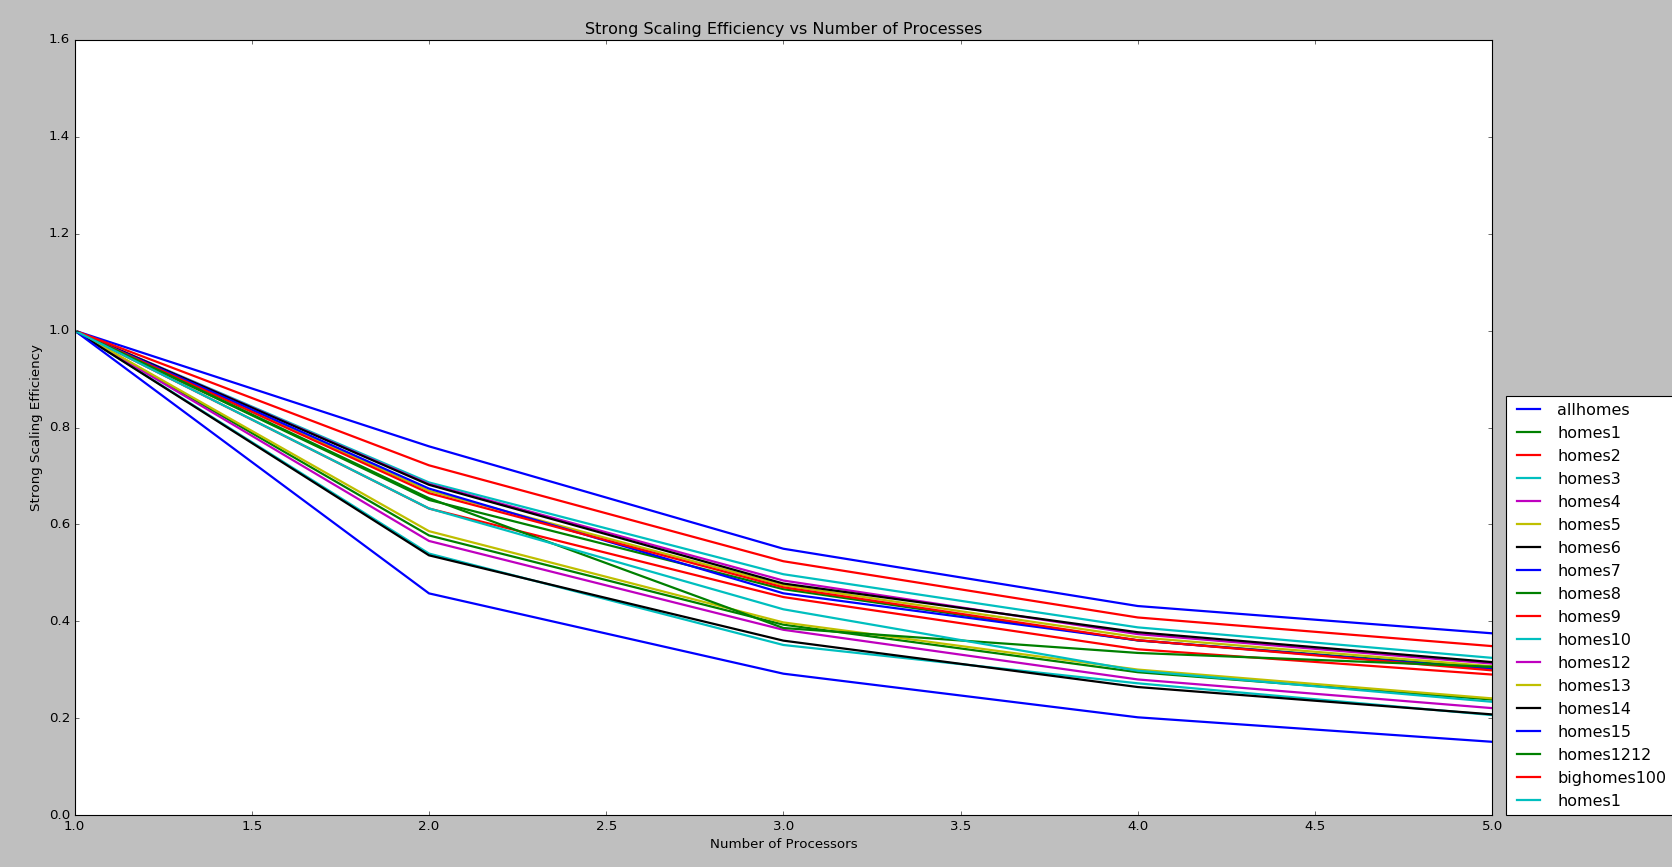
\includegraphics[width=8.5cm]{img/StrongScalingAllFiles}}
				\caption{Strong Scaling Efficiencies of All Files on RabinCDC}
				\label{fig:strongscale}
	\end{figure}
		\begin{figure}
			\centerline{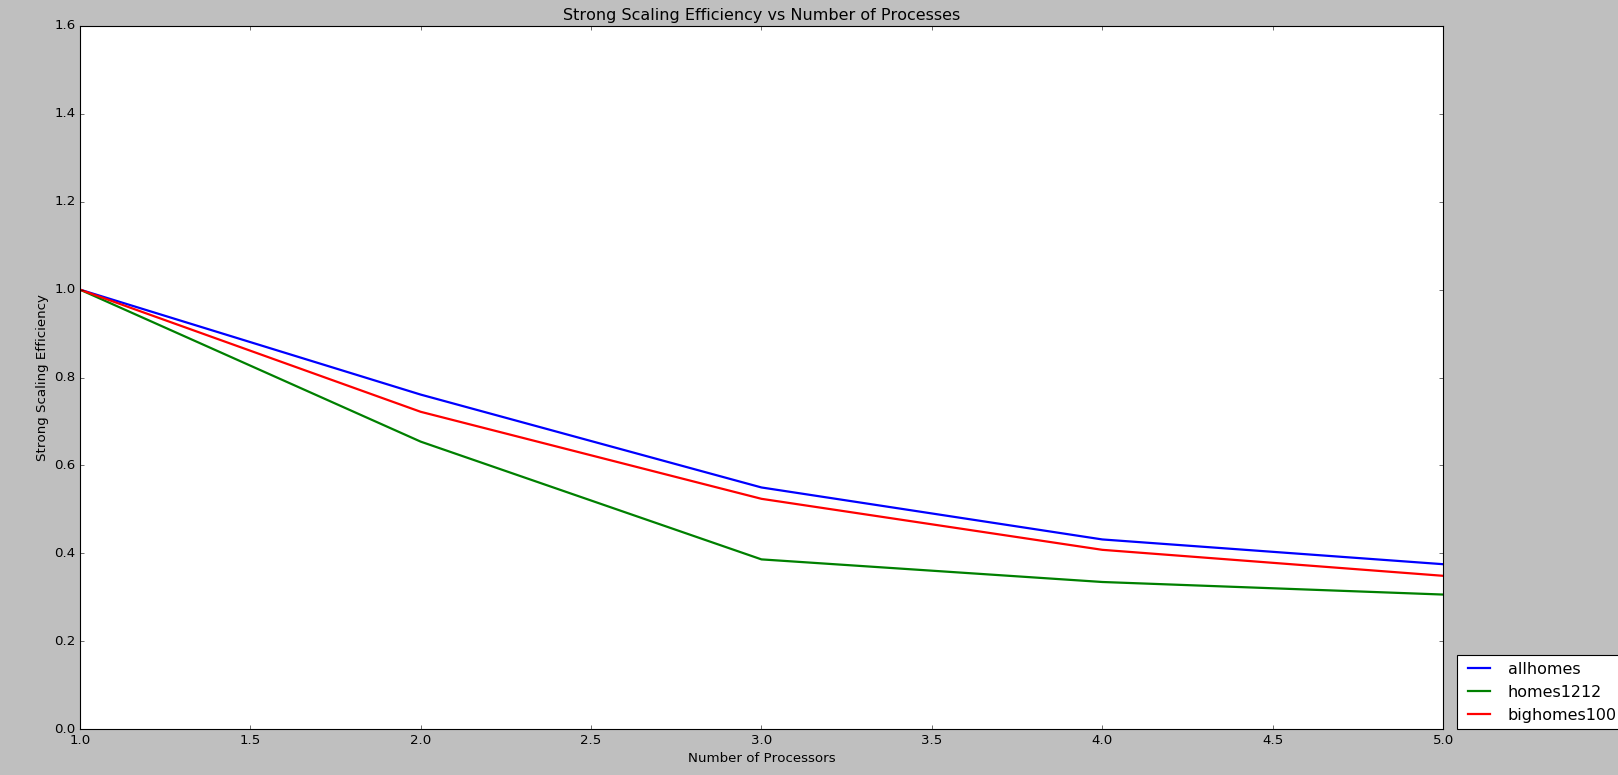
\includegraphics[width=8.5cm]{img/StrongScalingLargeFile}}
			\caption{Strong Scaling Efficiencies on Large Files}
			\label{fig:strongscalelarge}
		\end{figure}
	From our results, we see an overall decreasing trend of runtime at the larger file sizes from Figure 1. This is a notable result since it shows with simple parallelization that decent performance gains can be made. However, we note that the performance improvements are relatively minor.
	
	When running tests on small data files (number of lines less than 1 million), there were no significant improvements in the runtimes. In fact for the very small files, there were adverse effects on the run time. We believe these results are due to the fact that at these small file sizes, the benefit of using multiple processes is outweighed by the cost of spawning said processes. This may indicate that parallelizing RabinCDC for small file sizes is not optimal, and may in fact incur a cost.\\
	
	In contrast, there seem to be a clear benefit to parallelizing RabinCDC at large file sizes. Particularly for homes3, and homes1212, which had 2.5 million lines and 3.5 million lines respectively, there were great improvements. We see on the system we tested on that we were able to reduce the run time of RabinCDC to about 60\% of the serial run time. This shows great improvement since parallelizing with the \texttt{multiprocessing} module was relatively simple. This implies that any code can be parallelized with ease and great benefit. As we can see Figure 1, the run time noticeably decreases when increasing the number of processes. 
	
	Interestingly, when we compare the strong scaling factor of the most noticeable improvements, we see that the scaling efficiency actually decreases as we increase the number of processes. These lines are the lower lines in Figure 2 which have been highlighted in Figure 3. We believe that this is due to our system limitations, and that if our system had more cores, we would see a better strong scaling factor for more processes. Still, the benefits of parallelizing are clear even with a system limit of 2 cores. We believe including more cores would show even better benefits to parallelization and run time. 
	
	\subsection{Weak Scaling Efficiencies}
		\begin{figure}
			\centerline{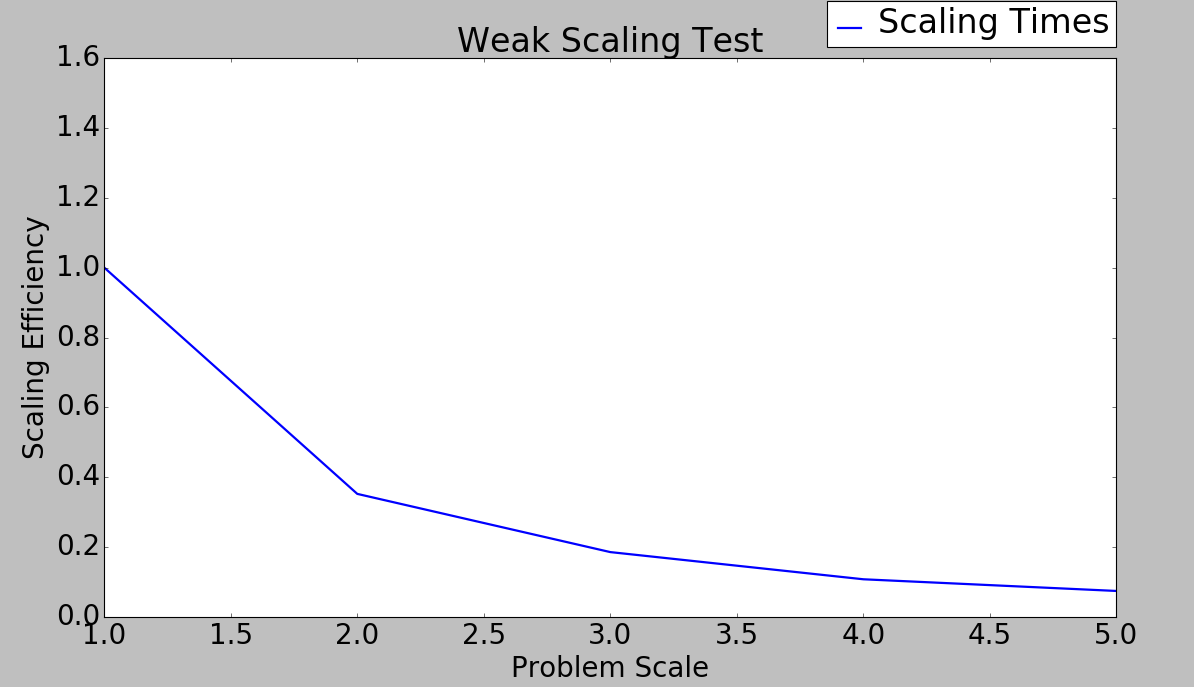
\includegraphics[width=8.5cm]{img/WeakScalingOnly}}
			\caption{Weak Scaling Efficiencies}
			\label{fig:weakscaleonly}
		\end{figure}

	Since synthetically creating trace data allowed us to specify the file sizes we wanted, we mostly focused on testing weak scaling efficiency since we could accurately scale the size of the files to the number of processes we used for the test. 
	
	On Figure 4, we see a clear decrease in the Weak Scaling Efficiency of our algorithm as we increase the size of the problem scale. This indicates that a parallel RabinCDC does not scale well with a larger problem size and more processes. This would mean that RabinCDC may not be the optimal algorithm to run on supercomputers like Comet since for the larger files that it will likely run, it will not show as much of a benefit in run time. We hypothesize that the decreased efficiency may be due to the larger sizes of data that the algorithm has to communicate across processes when first allocating the data and when aggregating the results. These increases in communication time are detrimental to the performance of the algorithm, and we attempted to avoid these communications by making our data global. However, this also introduced other inefficiencies, such as having to lock the data when a process accesses the array of data. Additionally, we had to introduce the \texttt{queue} data manager, so that we can pool the results in a thread-safe manner. 
	
	Given that we kept a constant ratio of 1 million lines per process and that the strong scaling efficiency decreased as we increased the number of processes, these results may not be fully indicative of how well our algorithm behaves as we increase the problem size and the number of processes. These results are still significant for average individuals who may not have access to supercomputers and would like to parallelize algorithms on personal computers, which have specifications comparable to the system we used for testing. 
	
	\section{Conclusions}
			\begin{figure}
				\centerline{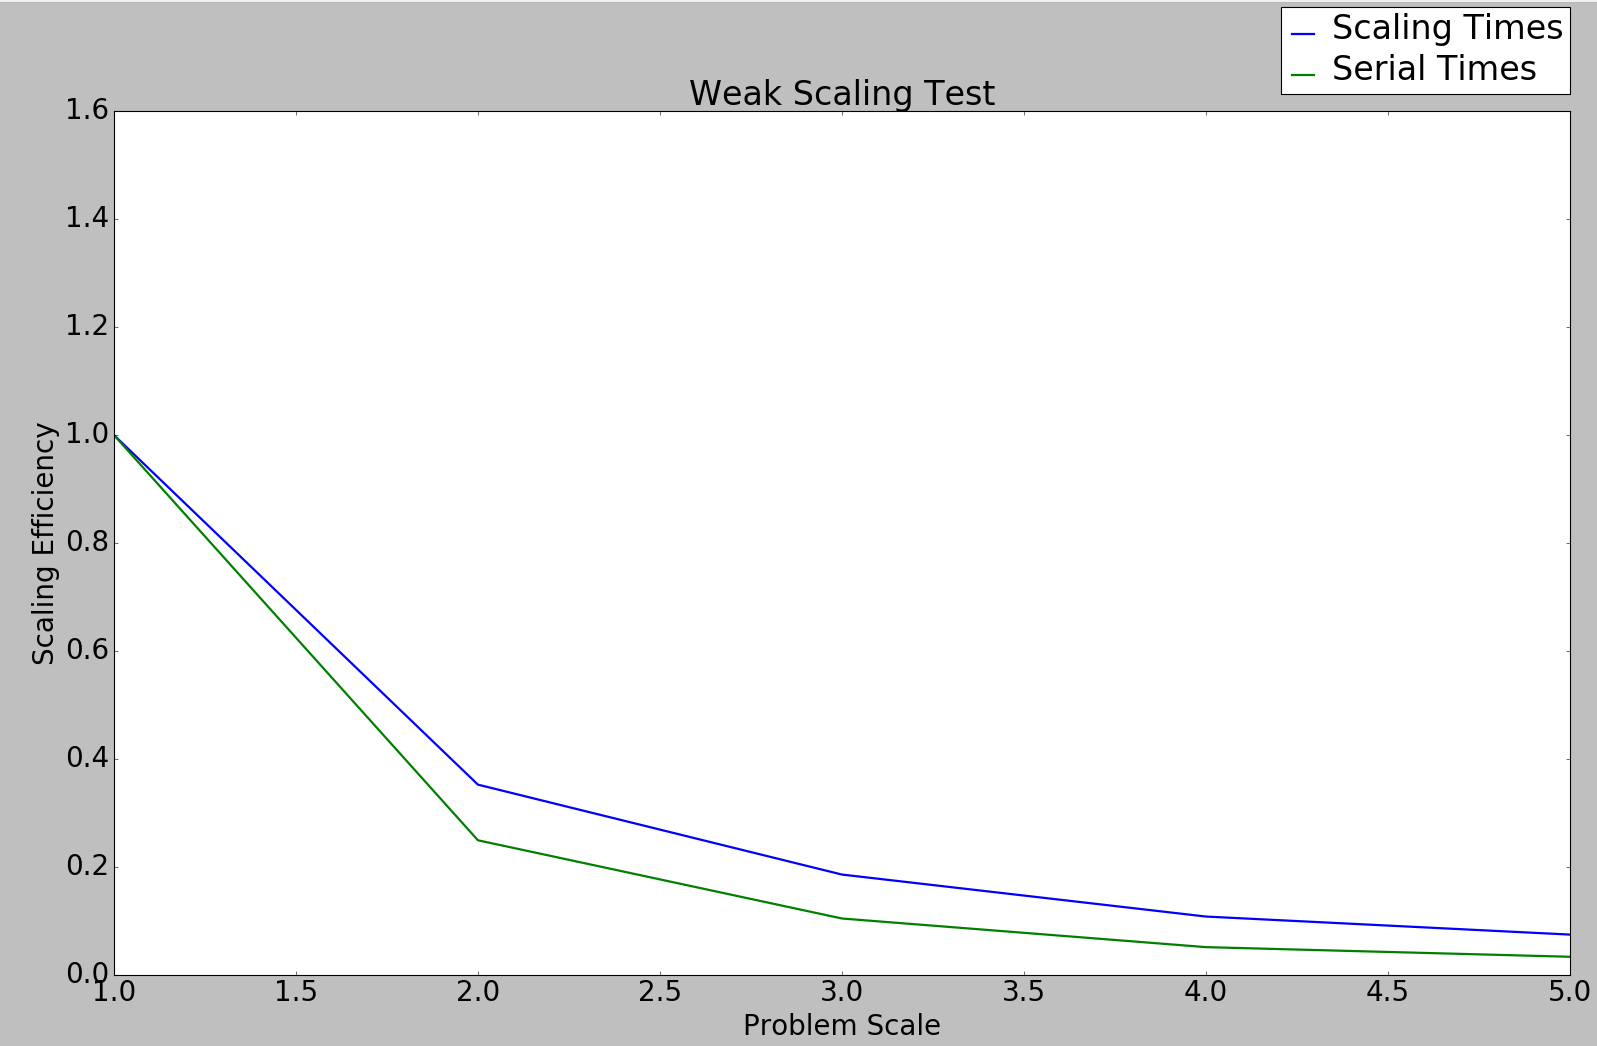
\includegraphics[width=8.5cm]{img/WeakScaling}}
				\caption{Weak Scaling Efficiencies}
				\label{fig:weakscale}
			\end{figure}
	We were able to obtain significant improvement of the run time in our context defined chunking algorithms by parallelizing them using the Python3 \texttt{multiprocessing} module. At large file sizes, we saw speedups of up to 40\% reduction in the amount of time required to process the file when using 5 processes. This may imply that the benefits of parallelization quickly reach their limit on personal systems such as the laptop we tested on. While supercomputing centers like the one at San Diego will probably see benefits including many more processes, this is still an important result as it shows that any individual can potentially introduce significant run time improvements to their code using the \texttt{multiprocessing} module in Python. \\
	
	When we graph the strong scaling efficiency vs number of processes in Figure 3, we see that there is a larger decrease in strong scaling efficiency for the larger file sizes. Since we are using the \texttt{multiprocessing} module in Python, the module just spawns new processes with specific sections of the data to work on. This result would be obvious when considering the purpose of the Python module we used. Since it just spawns new processes, eventually the results showcase more the effectiveness of the system's task scheduler than the benefits of parallelization. As a result, it is clear that there are diminishing returns for spawning new processes, which impacts the possible benefits of parallelization. Despite this, we still saw benefits that indicate parallelization is still a worthwhile venture. \\
	
	As for our weak scaling efficiency, we do not notice that much of an improvement over time. In fact the run time when we run N processing elements distributed to N processes is much worse than just one processing element distributed to one process. We believe that this discrepancy is due to the more costly data transfer costs incurred when allocating the large file into its separate processes. This highlights the costly nature of communication and data synchronization when parallelizing algorithms.\\

	
	Unfortunately, the Big O runtime of our algorithms were still O(n). Though this makes sense when analyzing the purpose of parallelization, which only splits up the work among many processes, so increasing the workload still increases the processing time linearly, just by a lesser amount than if we ran the code in serial. 
	
	Our results have shown that parallelization can provide valuable improvements to CDC algorithms. While the improvements may not scale as well on individual computers, we believe that our results show promising results for its effectiveness on super computers. We hope to continue our work with further testing on the weak scaling efficiencies of our parallel RabinCDC, and possibly testing on Comet if they ever update to 64-bit Python. 

	\section{Further Work}
	In the future, we will ideally test our algorithms on Comet, San Diego's Super Computer, for more intensive tests. We had initially planned on running our tests on Comet, but there were some system limitations that prohibited us from testing the scenarios that would be best run on Comet. One, Comet runs 32-bit Python 2.66, which limits the amount of RAM we can use while running RabinCDC. Due to our RabinCDC implementation, we required a 64-bit Python version, so that we could utilize more RAM. This would also produce conflicting results since the 32-bit limit would impact the stress tests that we had planned. Comet's main benefit would be the ability to test very large files, but the 32-bit limit would severely reduce the capability of Python to parse through these files. However from our initial tests on comet, we still recorded significant run time improvements for up to 20 processes. At that point with the file sizes we tested, we ran into the same limitation where the time it took to spawn the processes took a significant portion of the runtime, which greatly reduced the scaling efficiencies. 
	
	Additionally, our development environment was in Python 3.52, so if we wanted to test on Comet, we would need to check for compatibility. We would not be sure how this would impact our testing, so we chose to avoid this unnecessary complication by not using Comet.
	
	Lastly, since we were running different versions of Python, we could not guarantee that the \texttt{multiprocessing} module would perform identically across different versions, so we would not be confident that the results Comet produced would be valid. Thus, with all these considerations in mind, we chose not to test on Comet since we were unable to test the conditions that Comet would be best to use for testing.
	
	However, we would still like to perform large tests with Comet, so we would ideally test on Comet in the future if its Python version is updated to a 64-bit version. This would allow us to test a larger variety of conditions. Even if we do not test on Comet, we plan on continuing tests with a better system that has more cores, so that we can clearly see the benefits of parallelization. Since the \texttt{multiprocessing} module only spawns more processes, the breakpoint at which we become limited by the system's task scheduler is reached relatively quickly on our testing system (at about 5 processes). We had planned to graph our data over a larger x-axis range by testing a stronger desktop computer, but the system's Python environment was not compatible with the code we had written.
	
	Another possibility of more in-depth testing would be to test a larger variety of algorithms, possible even parallelizing AECDC as well, so that we can see how effective parallelization can be for slow algorithms. With the possibility of parallelization, it might bring up other algorithms that were deemed slow, and allow them to compete with FastCDC. Given our results, we have shown that even basic parallel processing will produce significant improvements in runtime, so some algorithms which may have terrible serial runtime compared to FastCDC can perform as effectively when parallelized. 
	
	As for other methods of parallelization, we looked into the \texttt{threading} module that Python 3 has, but we did not see enough significant benefits to justify further testing. One interesting note is that for small file sizes, the \texttt{threading} module outperformed the \texttt{multiprocessing} module. This is likely due to the much smaller overhead of spawning new threads instead of spawning processes. However, at larger file sizes, multi-threading did not show much improvement over the serial code, so we decided against using it. 
	
	There also exists the possibility of utilizing \texttt{Cython} or \texttt{pymp}. Cython would allow us to easily port Python code to faster C code, and allow us to bypass the global interpreter lock of Python, so we can attempt multi-threading. Pymp is a Python version of OpenMP, which would be interesting to test, since it would showcase the effectiveness of well known parallelization package that has been ported to Python. 
	  \begin{thebibliography}{1}
	  
	  \bibitem{notes} [1] Wen et al. “FastCDC: a Fast and Efficient Content-Defined Chunking Approach for Data Deduplication.” USENIX Annual Technical Conference (USENIC ATC ’16), Jan. 2016, www.usenix.org/system/files/conference/atc16/atc16-paper-xia.pdf. \\

	  \bibitem{notes} [2] Muthitacharoen, Athicha et al. “A Low-Bandwidth Network File System.” Proceedings of the Eighteenth ACM Symposium on Operating Systems Principles - SOSP '01, 2001, doi:10.1145/502051.502052. \\

	  \bibitem{notes} [3] Quinlan, Sean, and Sean Dorward. “Venti: a New Approach to Archival Storage.” Proceedings of USENIX Conference on File and Storage Technologies (FAST’02), Jan. 2002. \\

	  \bibitem{notes} [4] Zhang, Yucheng et al. “AE: An Asymmetric Extremum Content Defined Chunking Algorithm for Fast and Bandwidth-Efficient Data Deduplication.” 2015 IEEE Conference on Computer Communications (INFOCOM), 2015, doi:10.1109/infocom.2015.7218510. \\

	  \end{thebibliography}

	
		
	\end{document}
	% End of v2-acmtog-sample.tex (March 2012) - Gerry Murray, ACM
